\documentclass[preview,border=4mm,convert={density=600,outext=.png}]{standalone}
 
\usepackage{url}
\usepackage{times}
\usepackage{tikz}
\usetikzlibrary{fadings}
\usepackage{color}
\begin{document}
 

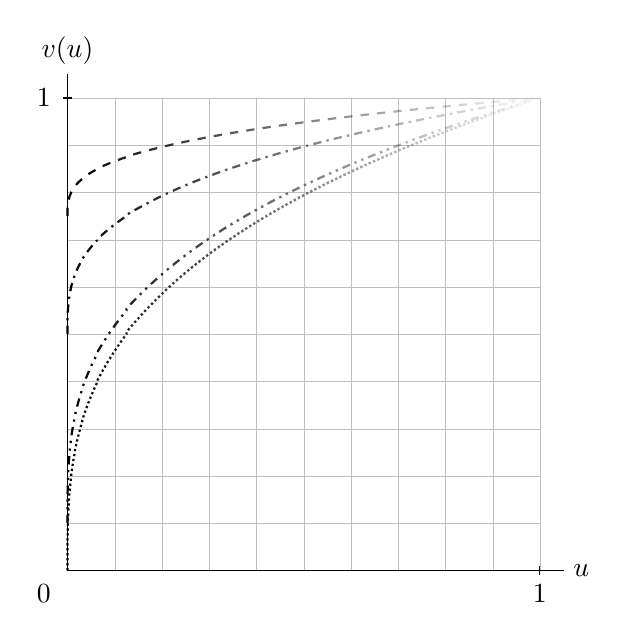
\begin{tikzpicture}[domain=0:1, scale=6] 
\draw[xstep=.1,ystep=.1,lightgray,ultra thin] (0,0) grid (1,1);
\draw (0,0) -- (1.05,0) node[right] {$u$}; 
\draw (0,0) -- (0,1.05) node[above] {$v(u)$};
\node at (-0.05,-0.05) {$0$};
\draw (-0.01,1) -- (0.01,1);
\node at (-0.05, 1) {$1$};
\draw (1,-0.01) -- (1,0.01);
\node at (1, -0.05) {$1$};
\draw[thick, dashdotdotted, path fading=east, domain=0:1,samples=9000] plot (\x,{0.1+0.9*(\x)^(1/3)});
%\node[color=red, right, align=left] at (0.61,0.25) {$v_0 = 0.1$};
\draw[thick, dashdotted, path fading=east,domain=0:1,samples=9000] plot (\x,{0.5+0.5*(\x)^(1/3)});
%\node[color=blue, right, align=left] at (0.61, 0.35) {$v_0 = 0.5$};
\draw[thick, dashed, path fading=east,domain=0:1,samples=9000] plot (\x,{0.75+0.25*(\x)^(1/3)});
%\node[color=orange, right, align=left] at (0.61, 0.45){$v_0 = 0.75$};
\draw[thick, densely dotted, path fading=east,domain=0:1,samples=9000] plot (\x,{(\x)^(1/3)});
\end{tikzpicture}

\end{document}